\documentclass{standalone}
\usepackage{tikz}
\usetikzlibrary{patterns, positioning}


\begin{document}
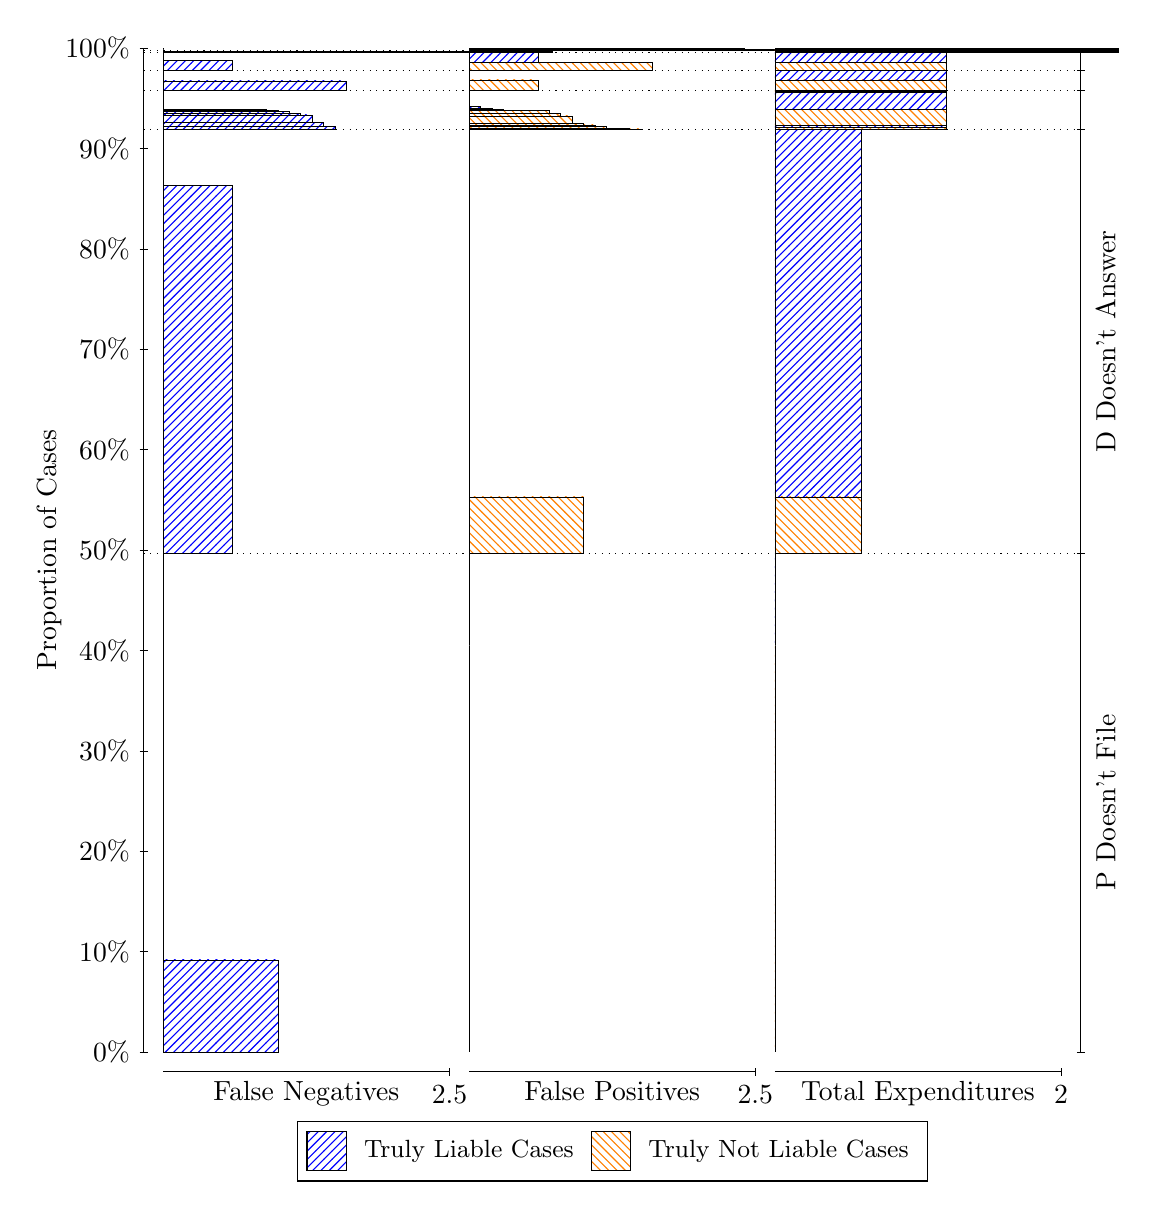
\begin{tikzpicture}
\draw[black, very thin] (1.5,1.75) -- (1.5,14.5);
\node[rotate=90, text=black, anchor=center] at (0.3, 8.125) {Proportion of Cases};
\draw[black, very thin] (1.45,1.75) -- (1.55,1.75);
\node[text=black, anchor=east] at (1.45, 1.75) {0\%};
\draw[black, very thin] (1.45,3.025) -- (1.55,3.025);
\node[text=black, anchor=east] at (1.45, 3.025) {10\%};
\draw[black, very thin] (1.45,4.3) -- (1.55,4.3);
\node[text=black, anchor=east] at (1.45, 4.3) {20\%};
\draw[black, very thin] (1.45,5.575) -- (1.55,5.575);
\node[text=black, anchor=east] at (1.45, 5.575) {30\%};
\draw[black, very thin] (1.45,6.85) -- (1.55,6.85);
\node[text=black, anchor=east] at (1.45, 6.85) {40\%};
\draw[black, very thin] (1.45,8.125) -- (1.55,8.125);
\node[text=black, anchor=east] at (1.45, 8.125) {50\%};
\draw[black, very thin] (1.45,9.4) -- (1.55,9.4);
\node[text=black, anchor=east] at (1.45, 9.4) {60\%};
\draw[black, very thin] (1.45,10.675) -- (1.55,10.675);
\node[text=black, anchor=east] at (1.45, 10.675) {70\%};
\draw[black, very thin] (1.45,11.95) -- (1.55,11.95);
\node[text=black, anchor=east] at (1.45, 11.95) {80\%};
\draw[black, very thin] (1.45,13.225) -- (1.55,13.225);
\node[text=black, anchor=east] at (1.45, 13.225) {90\%};
\draw[black, very thin] (1.45,14.5) -- (1.55,14.5);
\node[text=black, anchor=east] at (1.45, 14.5) {100\%};

\draw[black, very thin] (13.4,1.75) -- (13.4,14.5);
\draw[black, very thin] (13.35,1.75) -- (13.45,1.75);
\node[anchor=west] at (13.35, 1.75) {};
\draw[black, very thin] (13.35,8.086) -- (13.45,8.086);
\node[anchor=west] at (13.35, 8.086) {};
\draw[black, very thin] (13.35,13.47) -- (13.45,13.47);
\node[anchor=west] at (13.35, 13.47) {};
\draw[black, very thin] (13.35,13.96) -- (13.45,13.96);
\node[anchor=west] at (13.35, 13.96) {};
\draw[black, very thin] (13.35,14.219) -- (13.45,14.219);
\node[anchor=west] at (13.35, 14.219) {};
\draw[black, very thin] (13.35,14.443) -- (13.45,14.443);
\node[anchor=west] at (13.35, 14.443) {};
\draw[black, very thin] (13.35,14.474) -- (13.45,14.474);
\node[anchor=west] at (13.35, 14.474) {};
\draw[black, very thin] (13.35,14.5) -- (13.45,14.5);
\node[anchor=west] at (13.35, 14.5) {};

\draw[black, very thin, pattern color=blue, pattern=north east lines] (1.75,1.75) rectangle (3.2033,2.9207);
\draw[black, very thin, pattern color=orange, pattern=north west lines] (1.75,2.9207) rectangle (1.75,8.086);
\draw[black, very thin, pattern color=blue, pattern=north east lines] (1.75,8.086) rectangle (2.622,12.758);
\draw[black, very thin, pattern color=orange, pattern=north west lines] (1.75,12.758) rectangle (1.75,13.47);
\draw[black, very thin, pattern color=blue, pattern=north east lines] (1.75,13.47) rectangle (3.93,13.509);
\draw[black, very thin, pattern color=blue, pattern=north east lines] (1.75,13.509) rectangle (3.7847,13.554);
\draw[black, very thin, pattern color=blue, pattern=north east lines] (1.75,13.554) rectangle (3.6393,13.652);
\draw[black, very thin, pattern color=blue, pattern=north east lines] (1.75,13.652) rectangle (3.494,13.671);
\draw[black, very thin, pattern color=blue, pattern=north east lines] (1.75,13.671) rectangle (3.3487,13.696);
\draw[black, very thin, pattern color=blue, pattern=north east lines] (1.75,13.696) rectangle (3.2033,13.712);
\draw[black, very thin, pattern color=blue, pattern=north east lines] (1.75,13.712) rectangle (3.058,13.72);
\draw[black, very thin, pattern color=blue, pattern=north east lines] (1.75,13.72) rectangle (2.9127,13.722);
\draw[black, very thin, pattern color=blue, pattern=north east lines] (1.75,13.722) rectangle (2.7673,13.725);
\draw[black, very thin, pattern color=orange, pattern=north west lines] (1.75,13.725) rectangle (1.75,13.96);
\draw[black, very thin, pattern color=blue, pattern=north east lines] (1.75,13.96) rectangle (4.0753,14.083);
\draw[black, very thin, pattern color=orange, pattern=north west lines] (1.75,14.083) rectangle (1.75,14.219);
\draw[black, very thin, pattern color=blue, pattern=north east lines] (1.75,14.219) rectangle (2.622,14.347);
\draw[black, very thin, pattern color=orange, pattern=north west lines] (1.75,14.347) rectangle (1.75,14.443);
\draw[black, very thin, pattern color=blue, pattern=north east lines] (1.75,14.443) rectangle (6.6913,14.453);
\draw[black, very thin, pattern color=orange, pattern=north west lines] (1.75,14.453) rectangle (1.75,14.474);
\draw[black, very thin, pattern color=orange, pattern=north west lines] (1.75,14.474) rectangle (1.75,14.483);
\draw[black, very thin, pattern color=blue, pattern=north east lines] (1.75,14.483) rectangle (1.75,14.5);
\draw[black, very thin, pattern color=orange, pattern=north west lines] (5.6333,1.75) rectangle (5.6333,6.9153);
\draw[black, very thin, pattern color=blue, pattern=north east lines] (5.6333,6.9153) rectangle (5.6333,8.086);
\draw[black, very thin, pattern color=orange, pattern=north west lines] (5.6333,8.086) rectangle (7.0867,8.7983);
\draw[black, very thin, pattern color=blue, pattern=north east lines] (5.6333,8.7983) rectangle (5.6333,13.47);
\draw[black, very thin, pattern color=orange, pattern=north west lines] (5.6333,13.47) rectangle (7.8133,13.473);
\draw[black, very thin, pattern color=orange, pattern=north west lines] (5.6333,13.473) rectangle (7.668,13.476);
\draw[black, very thin, pattern color=orange, pattern=north west lines] (5.6333,13.476) rectangle (7.5227,13.483);
\draw[black, very thin, pattern color=orange, pattern=north west lines] (5.6333,13.483) rectangle (7.3773,13.5);
\draw[black, very thin, pattern color=orange, pattern=north west lines] (5.6333,13.5) rectangle (7.232,13.523);
\draw[black, very thin, pattern color=orange, pattern=north west lines] (5.6333,13.523) rectangle (7.0867,13.543);
\draw[black, very thin, pattern color=orange, pattern=north west lines] (5.6333,13.543) rectangle (6.9413,13.638);
\draw[black, very thin, pattern color=orange, pattern=north west lines] (5.6333,13.638) rectangle (6.796,13.671);
\draw[black, very thin, pattern color=orange, pattern=north west lines] (5.6333,13.671) rectangle (6.6507,13.705);
\draw[black, very thin, pattern color=blue, pattern=north east lines] (5.6333,13.705) rectangle (6.36,13.708);
\draw[black, very thin, pattern color=blue, pattern=north east lines] (5.6333,13.708) rectangle (6.2147,13.71);
\draw[black, very thin, pattern color=blue, pattern=north east lines] (5.6333,13.71) rectangle (6.0693,13.718);
\draw[black, very thin, pattern color=blue, pattern=north east lines] (5.6333,13.718) rectangle (5.924,13.734);
\draw[black, very thin, pattern color=blue, pattern=north east lines] (5.6333,13.734) rectangle (5.7787,13.759);
\draw[black, very thin, pattern color=blue, pattern=north east lines] (5.6333,13.759) rectangle (5.6333,13.96);
\draw[black, very thin, pattern color=orange, pattern=north west lines] (5.6333,13.96) rectangle (6.5053,14.096);
\draw[black, very thin, pattern color=blue, pattern=north east lines] (5.6333,14.096) rectangle (5.6333,14.219);
\draw[black, very thin, pattern color=orange, pattern=north west lines] (5.6333,14.219) rectangle (7.9587,14.315);
\draw[black, very thin, pattern color=blue, pattern=north east lines] (5.6333,14.315) rectangle (6.5053,14.443);
\draw[black, very thin, pattern color=orange, pattern=north west lines] (5.6333,14.443) rectangle (5.6333,14.464);
\draw[black, very thin, pattern color=blue, pattern=north east lines] (5.6333,14.464) rectangle (5.6333,14.474);
\draw[black, very thin, pattern color=orange, pattern=north west lines] (5.6333,14.474) rectangle (10.575,14.483);
\draw[black, very thin, pattern color=blue, pattern=north east lines] (5.6333,14.483) rectangle (9.1213,14.5);
\draw[black, very thin, pattern color=orange, pattern=north west lines] (9.5167,1.75) rectangle (9.5167,6.9153);
\draw[black, very thin, pattern color=blue, pattern=north east lines] (9.5167,6.9153) rectangle (9.5167,8.086);
\draw[black, very thin, pattern color=orange, pattern=north west lines] (9.5167,8.086) rectangle (10.607,8.7983);
\draw[black, very thin, pattern color=blue, pattern=north east lines] (9.5167,8.7983) rectangle (10.607,13.47);
\draw[black, very thin, pattern color=orange, pattern=north west lines] (9.5167,13.47) rectangle (11.697,13.493);
\draw[black, very thin, pattern color=blue, pattern=north east lines] (9.5167,13.493) rectangle (11.697,13.518);
\draw[black, very thin, pattern color=orange, pattern=north west lines] (9.5167,13.518) rectangle (11.697,13.72);
\draw[black, very thin, pattern color=blue, pattern=north east lines] (9.5167,13.72) rectangle (11.697,13.939);
\draw[black, very thin, pattern color=orange, pattern=north west lines] (9.5167,13.939) rectangle (11.697,13.95);
\draw[black, very thin, pattern color=blue, pattern=north east lines] (9.5167,13.95) rectangle (11.697,13.96);
\draw[black, very thin, pattern color=orange, pattern=north west lines] (9.5167,13.96) rectangle (11.697,14.096);
\draw[black, very thin, pattern color=blue, pattern=north east lines] (9.5167,14.096) rectangle (11.697,14.219);
\draw[black, very thin, pattern color=orange, pattern=north west lines] (9.5167,14.219) rectangle (11.697,14.315);
\draw[black, very thin, pattern color=blue, pattern=north east lines] (9.5167,14.315) rectangle (11.697,14.443);
\draw[black, very thin, pattern color=orange, pattern=north west lines] (9.5167,14.443) rectangle (13.877,14.464);
\draw[black, very thin, pattern color=blue, pattern=north east lines] (9.5167,14.464) rectangle (13.877,14.474);
\draw[black, very thin, pattern color=orange, pattern=north west lines] (9.5167,14.474) rectangle (13.877,14.483);
\draw[black, very thin, pattern color=blue, pattern=north east lines] (9.5167,14.483) rectangle (13.877,14.5);
\draw[black, dotted] (1.5,8.086) -- (13.4,8.086);
\draw[black, dotted] (1.5,13.47) -- (13.4,13.47);
\draw[black, dotted] (1.5,13.96) -- (13.4,13.96);
\draw[black, dotted] (1.5,14.219) -- (13.4,14.219);
\draw[black, dotted] (1.5,14.443) -- (13.4,14.443);
\draw[black, dotted] (1.5,14.474) -- (13.4,14.474);
\draw[black, very thin] (1.75,1.5) -- (5.3833,1.5);
\node[text=black, anchor=north] at (3.5667, 1.5) {False Negatives};
\draw[black, very thin] (5.3833,1.45) -- (5.3833,1.55);
\node[text=black, anchor=north] at (5.3833, 1.45) {2.5};

\draw[black, very thin] (5.6333,1.5) -- (9.2667,1.5);
\node[text=black, anchor=north] at (7.45, 1.5) {False Positives};
\draw[black, very thin] (9.2667,1.45) -- (9.2667,1.55);
\node[text=black, anchor=north] at (9.2667, 1.45) {2.5};

\draw[black, very thin] (9.5167,1.5) -- (13.15,1.5);
\node[text=black, anchor=north] at (11.333, 1.5) {Total Expenditures};
\draw[black, very thin] (13.15,1.45) -- (13.15,1.55);
\node[text=black, anchor=north] at (13.15, 1.45) {2};

\node[text=black, centered, rotate=90] at (13.72, 4.918) {P Doesn't File};
\node[text=black, centered, rotate=90] at (13.72, 10.778) {D Doesn't Answer};






\draw (7.449999999999999,1.5) node[draw=none] (baseCoordinate) {};
\begin{scope}[align=center]
        \matrix[scale=0.5, draw=black, below=0.5cm of baseCoordinate, nodes={draw}, column sep=0.1cm]{
            \node[rectangle, draw, minimum width=0.5cm, minimum height=0.5cm, pattern color=blue, pattern=north east lines] {}; &
            \node[draw=none, font=\small, text=black] (B) {Truly Liable Cases}; &
            \node[rectangle, draw, minimum width=0.5cm, minimum height=0.5cm, pattern color=orange, pattern=north west lines] {}; &
            \node[draw=none, font=\small, text=black] (B) {Truly Not Liable Cases}; \\
            };
\end{scope}

\end{tikzpicture}
\end{document}